% !TEX root = ../main.tex

\chapter{综合实验设计与结果分析}

\section{实验环境与软硬件配置}

本章的作用是把前文提出的系统路线放到统一实验框架中检验：FlashTOD 是否在真实或半真实金融数据上保持可用，单卡优化是否确实压缩了数据路径，多 GPU 扩展是否把吞吐提升建立在合理的结构选择之上，以及 I/O 路径与归并方式在何种条件下开始成为新的限制因素。围绕这些问题，本节先交代实验所依赖的硬件条件、软件栈和实验分类口径。

硬件环境方面，实验平台由多张同型号 GPU、主机 CPU、内存、SSD 以及对应 PCIe 拓扑组成。单卡实验使用 1 张 GPU 运行完整的候选召回与异常评分链路，主要观察第四章提出的数据路径优化、异步流组织、RAPIDS 后端重构、FAISS-GPU 前期接口验证经验和 FlashANNS 候选召回前端接入在单设备上的综合表现；多卡实验使用 2 张及以上 GPU，主要对应第五章中的索引复制（replicated）扩展、控制面调度、设备侧归并和 I/O 通道控制。由于本文后续还需要讨论拓扑差异对扩展结果的影响，GPU 型号、显存容量、CPU 型号、主机内存、SSD 容量、PCIe 代际和 NUMA 关系都需要作为实验前提显式给出。

软件环境方面，实验系统由 PyTOD 评分实现、FlashANNS 候选召回前端、FAISS-GPU 初步 ANN 接口验证组件、RAPIDS 数据处理与资源管理组件、多 GPU 通信和调度运行时共同组成。FAISS-GPU 主要用于验证候选召回接口、设备侧输入输出路径和候选结果格式，完整 FlashTOD 路径中的大规模候选生成以后续接入的 FlashANNS 为主。为了保证结果可复核，本文固定 Python、PyTorch、PyTOD、FAISS-GPU、CUDA、NCCL 以及操作系统版本；CuPy、cuDF、cuML、RMM 等 GPU 数据处理与资源管理组件的版本也一并记录为统一软件环境快照。

在实验分类上，本文将综合实验划分为三组：方法有效性验证实验，对应真实或半真实数据及 1M 合成桥接口径；单卡系统性能实验，沿第三章定义的单卡规模链路组织；多 GPU 扩展实验则在此基础上延伸至 100M 样本压力场景，用于比较索引复制主方案、设备侧归并兜底路径以及 I/O 路径组织方式。三类实验共享一套基础代码框架，但在数据规模、硬件使用方式和评价重点上各有分工。

表~\ref{tab:hw-config} 给出了实验平台与软件环境配置快照，图~\ref{fig:exp-topology} 则补充展示了实验平台中 CPU、GPU、SSD 与 PCIe/NUMA 的连接关系，为后续性能差异解释提供硬件背景。

\begin{table}[htbp]
  \caption{实验平台与软件环境配置}
  \label{tab:hw-config}
  \centering
  \small
  \renewcommand{\arraystretch}{1.15}
  \begin{adjustbox}{max width=\linewidth}
  \begin{tabular}{P{2.3cm}P{5.8cm}P{6.2cm}}
    \toprule
    项目 & 规格 & 说明 \\
    \midrule
    \multicolumn{3}{l}{\textbf{硬件平台配置}} \\
    \midrule
    CPU 平台 & 2 $\times$ Intel Xeon Gold 6348 @ 2.60GHz & 56 核 112 线程，双 NUMA \\
    主存容量 & 503\,GiB & 系统总内存 \\
    GPU 平台 & 8 $\times$ NVIDIA GeForce RTX 3090 & 24\,GB/卡，总显存 192\,GB \\
    PCIe 能力 & PCIe Gen4 $\times$16 & 8 张 GPU 均为 Gen4 $\times$16 \\
    本地存储 & 3 $\times$ NVMe SSD & 894.3\,GB $\times$ 2，3.5\,TB $\times$ 1，总约 5.29\,TB \\
    NUMA 拓扑 & 2 个 NUMA 节点 & NUMA 0 对应 GPU0--GPU3，NUMA 1 对应 GPU4--GPU7 \\
    GPU 互连特征 & 同侧 PIX/PXB，跨侧 SYS & 用于解释多 GPU 与 I/O 通道实验 \\
    网络接口 & 2 $\times$ Mellanox NIC & mlx5\_0，mlx5\_1 \\
    \midrule
    \multicolumn{3}{l}{\textbf{软件环境配置}} \\
    \midrule
    操作系统 & Ubuntu 20.04.4 LTS，Linux 5.13.0-30-generic & 实验运行环境 \\
    Python / CUDA & Python 3.11.14；CUDA Runtime 12.4 & 基础运行时环境 \\
    深度学习框架 & PyTorch 2.5.0+cu124；NCCL 2.21.5 & GPU 张量计算与通信环境 \\
    驱动环境 & NVIDIA Driver 550.120 & 与 CUDA 12.4 对应 \\
    异常检测框架 & PyTOD（\href{https://github.com/yzhao062/pytod}{yzhao062/pytod}） &  GitHub 主仓库默认分支 main \\
    ANN 检索组件 & FlashANNS / ann\_search（\href{https://github.com/Tinkerver/ann_search}{Tinkerver/ann\_search}） & GitHub 主仓库默认分支 main \\
    其他核心库 & FAISS 1.13.2；PyOD 2.0.6；NumPy 2.2.6；SciPy 1.13.1；scikit-learn 1.6.1 & 实验所用主要 Python 依赖；FAISS 用于初步 ANN 接口验证和对照实现 \\
    RAPIDS 相关 & CuPy 13.3.0；cuDF 25.02.00；cuML 25.02.00；RMM 25.02.00 & 用于 GPU 侧表格处理、中间结果组织、数组计算和内存资源管理，不单独归因整体性能收益 \\
    \bottomrule
  \end{tabular}
  \end{adjustbox}
\end{table}

\begin{figure}[!htbp]
  \centering
  % 图 6-1：黑白学术风格硬件拓扑示意图（Host—双 CPU/NUMA—GPU—NVMe）
  \resizebox{0.95\linewidth}{!}{%
  \begin{tikzpicture}[
    font=\small,
    >=Latex,
    box/.style={draw, line width=0.5pt, rounded corners=1pt, align=center, inner xsep=6pt, inner ysep=5pt},
    titlebox/.style={box, minimum width=9.5cm},
    cpbox/.style={box, minimum width=6.2cm, minimum height=2.2cm},
    gpubox/.style={box, minimum width=1.55cm, minimum height=1.25cm, inner xsep=3pt, inner ysep=3pt},
    ssdbox/.style={box, minimum width=13.2cm, minimum height=1.4cm},
    link/.style={draw, line width=0.5pt},
    alink/.style={link,-Latex},
  ]
    % 顶部 Host
    \node[titlebox] (host) {Host\\Ubuntu 20.04 / Driver 550};

    % 两个 CPU/NUMA 盒子
    \node[cpbox, below left=14mm and 12mm of host] (cpu0) {CPU Socket 0 / NUMA 0\\Xeon Gold 6348\\Memory $\sim$257.6\,GB};
    \node[cpbox, below right=14mm and 12mm of host] (cpu1) {CPU Socket 1 / NUMA 1\\Xeon Gold 6348\\Memory $\sim$258.0\,GB};

    % Host 到 CPU 的连接
    \draw[link] (host.south) -- ++(0,-6mm) -| (cpu0.north);
    \draw[link] (host.south) -- ++(0,-6mm) -| (cpu1.north);

    % CPU0 <-> CPU1 SYS/UPI
    \draw[<->, link] (cpu0.east) -- node[above, font=\footnotesize] {SYS / UPI} (cpu1.west);

    % GPU 行（左 4 右 4）
    \node[gpubox, below=12mm of cpu0.south west, anchor=north west] (gpu0) {GPU0\\RTX 3090\\24\,GB};
    \node[gpubox, right=4mm of gpu0] (gpu1) {GPU1\\RTX 3090\\24\,GB};
    \node[gpubox, right=4mm of gpu1] (gpu2) {GPU2\\RTX 3090\\24\,GB};
    \node[gpubox, right=4mm of gpu2] (gpu3) {GPU3\\RTX 3090\\24\,GB};

    \node[gpubox, below=12mm of cpu1.south west, anchor=north west] (gpu4) {GPU4\\RTX 3090\\24\,GB};
    \node[gpubox, right=4mm of gpu4] (gpu5) {GPU5\\RTX 3090\\24\,GB};
    \node[gpubox, right=4mm of gpu5] (gpu6) {GPU6\\RTX 3090\\24\,GB};
    \node[gpubox, right=4mm of gpu6] (gpu7) {GPU7\\RTX 3090\\24\,GB};

    % CPU 到 GPU 的连接（标注 PCIe Gen4 Fabric）
    \draw[alink] (cpu0.south) -- node[left, font=\footnotesize, align=center] {PCIe Gen4\\Fabric} ($(gpu0.north)!0.5!(gpu3.north)$);
    \draw[alink] (cpu1.south) -- node[right, font=\footnotesize, align=center] {PCIe Gen4\\Fabric} ($(gpu4.north)!0.5!(gpu7.north)$);

    % 底部共享 NVMe SSD Pool
    \node[ssdbox, below=14mm of $(gpu0.south)!0.5!(gpu7.south)$] (ssd) {Local NVMe SSD Pool\\894.3\,GB + 894.3\,GB + 3.5\,TB};

    % 从两侧 GPU 区域指向共享 SSD（示意共享存储池）
    \draw[link] ($(gpu0.south)!0.5!(gpu3.south)$) -- ($(gpu0.south)!0.5!(gpu3.south)$ |- ssd.north) -- (ssd.north);
    \draw[link] ($(gpu4.south)!0.5!(gpu7.south)$) -- ($(gpu4.south)!0.5!(gpu7.south)$ |- ssd.north) -- (ssd.north);
  \end{tikzpicture}%
  }
  \caption{实验平台拓扑示意图（本文根据实验平台配置绘制）}
  \label{fig:exp-topology}
\end{figure}

\section{数据集与任务设置}

本章沿用第三章的数据安排，但实验目的已经从建立系统对象转向统一验证系统结论，不同规模数据在这里承担的角色也更明确。真实或半真实金融数据对应全文的现实口径，1M 合成数据承担桥接层，单卡实验沿前述规模链路逐层展开，多 GPU 实验则继续延伸到 100M 样本压力场景。

需要说明的是，本章中的真实或半真实金融数据并不等同于金融机构生产系统中的在线原始流量，而是指经过公开发布、脱敏、匿名化、采样或特征变换后的金融相关任务数据。它们适合用于检验异常检测链路在真实业务语境下的可用性；10M、50M、100M 等 AMLSim / IBM AML 合成规模则主要服务于系统压力、吞吐扩展和 I/O 路径验证，相关结论应理解为在本文实验平台和生成口径下的工程趋势。

在有效性验证部分，本文继续使用 IEEE-CIS Fraud Detection、Credit Card Fraud Detection 和 DGraphFin 这三类具有代表性的公开金融数据，分别覆盖结构化支付风控、经典信用卡欺诈以及图金融数据场景。具体数据来源和字段特征已在第三章中给出，这里不再重复展开。

在系统性能与扩展实验部分，本文采用第三章已经介绍过的高保真合成金融交易数据。通过规模分层让不同规模分别承担不同验证任务，其中，1M 数据用于连接真实数据验证与系统实验，使检测效果和端到端实现处于同一实验口径；10M 数据是单卡综合性能与多 GPU 扩展的共同起点；50M 数据主要用于观察规模继续增大后单卡链路与多 GPU 扩展的中间趋势；100M 数据则主要服务于多 GPU 扩展、跨卡归并和共享路径冲突实验。

在任务组织上，本章实验可分为四类：候选召回与异常评分有效性任务、单卡性能任务、多 GPU 索引复制扩展任务以及跨卡归并与 I/O 路径任务。这些任务共享同一套核心实现，但比较对象和观测重点并不相同。有效性任务更关注检测结果与候选排序质量；单卡性能任务更关注数据路径压缩后的吞吐、延迟和利用率；多 GPU 任务则进一步考察索引复制主方案、设备侧归并兜底路径以及共享路径冲突对扩展收益的影响。

在数据使用方式上，有效性验证任务按训练集、验证集和测试集划分，以保证 PR-AUC、Recall@$k$ 等指标可比；性能与扩展实验则采用固定索引集与固定查询集，将查询批量持续注入系统，以更准确地衡量 QPS、延迟分位数与资源利用率。这样区分能够避免把检测效果评估和系统压测混在同一套数据口径下讨论。

图~\ref{fig:scale-vs-exp} 展示了规模层级与实验类型的映射。

\begin{figure}[!htbp]
  \centering
  \begin{tikzpicture}[
    font=\small,
    >=Latex,
    main/.style={draw, rounded corners=1pt, line width=0.4pt, align=center, inner sep=4pt, minimum width=1.8cm},
    child/.style={draw, line width=0.4pt, align=left, inner sep=3pt, text width=5.2cm},
    link/.style={-Latex, line width=0.4pt}
  ]
    % 主层级（自上而下）
    \node[main] (real) {真实集};
    \node[main, below=5mm of real] (m1) {1M};
    \node[main, below=20mm of m1] (m10) {10M};
    \node[main, below=12mm of m10] (m50) {50M};
    \node[main, below=10mm of m50] (m100) {100M};

    % 真实集 -> 2 子项
    \node[child, right=12mm of real, yshift=5mm] (real_a) {真实场景有效性验证};
    \node[child, below=2mm of real_a] (real_b) {单卡 / 多 GPU 真实口径基准};
    \draw[link] (real.east) -- (real_a.west);
    \draw[link] (real.east) -- (real_b.west);

    % 1M -> 3 子项
    \node[child, right=12mm of m1, yshift=1mm] (m1_a) {方法有效性桥接实验};
    \node[child, below=2mm of m1_a] (m1_b) {单卡性能起点实验};
    \node[child, below=2mm of m1_b] (m1_c) {多 GPU 性能起点实验};
    \draw[link] (m1.east) -- (m1_a.west);
    \draw[link] (m1.east) -- (m1_b.west);
    \draw[link] (m1.east) -- (m1_c.west);

    % 10M -> 2 子项
    \node[child, right=12mm of m10, yshift=2.5mm] (m10_a) {单卡系统性能实验};
    \node[child, below=2mm of m10_a] (m10_b) {多 GPU 索引复制扩展实验};
    \draw[link] (m10.east) -- (m10_a.west);
    \draw[link] (m10.east) -- (m10_b.west);

    % 50M -> 2 子项
    \node[child, right=12mm of m50, yshift=2.5mm] (m50_a) {单卡中大规模性能实验};
    \node[child, below=2mm of m50_a] (m50_b) {多 GPU 中大规模扩展实验};
    \draw[link] (m50.east) -- (m50_a.west);
    \draw[link] (m50.east) -- (m50_b.west);

    % 100M -> 1 子项
    \node[child, right=12mm of m100] (m100_a) {多 GPU 扩展与压力测试实验};
    \draw[link] (m100.east) -- (m100_a.west);
  \end{tikzpicture}
  \caption{数据规模层级与实验类型关系图（本文绘制）}
  \label{fig:scale-vs-exp}
\end{figure}

本章据此区分效果评估和系统压测：有效性口径沿用固定随机种子的训练/验证/测试划分，用于比较 PR-AUC、Recall@$k$ 与 Top-$k$ overlap；更大规模性能实验则固定索引集和查询集，持续注入请求以观察 QPS、p99 延迟和资源利用率。


\section{评价指标与比较原则}

本章采用的指标体系服务于全文的四条核心判断：FlashTOD 是否在效果上可接受，单卡优化是否主要压缩了数据路径，多 GPU 索引复制是否真正提升了吞吐，以及 I/O 路径是否决定扩展上限。围绕这四类判断，指标被组织为四组：异常检测效果指标、候选检索质量指标、系统吞吐与延迟指标以及资源利用率指标。

其中，受试者工作特征曲线下面积（Receiver Operating Characteristic Area Under Curve，ROC-AUC）、PR-AUC 与 Recall@$k$ 用于评价候选召回与张量化评分组合是否仍保持合理的检测能力；Recall@$k$ 与 Top-$k$ overlap 用于观察候选召回是否改变了最终排序口径；QPS、平均延迟与 p95/p99 延迟直接对应系统在单卡和多卡场景中的端到端收益；GPU 利用率、CPU 占用率、显存使用率、I/O 带宽利用率以及 CPU$\leftrightarrow$GPU 传输开销占比，则用于解释这些收益来自哪里。

金融异常样本通常远少于正常样本。此时 ROC 曲线中的假阳性率会被大量真负例稀释，单独使用 ROC-AUC 可能弱化对少数类识别质量的观察；Precision-Recall 曲线更直接地反映精确率与召回率之间的关系\citep{davis2006prroc,saito2015prauc}。因此，本文把 PR-AUC 作为主要效果指标之一，并与 Recall@$k$、Top-$k$ overlap 共同报告。这并不意味着 PR-AUC 在所有数据分布下都绝对优于 ROC-AUC，而是与本文类别不平衡和风险样本排序的评价目标更匹配。

比较时不将所有方案统称为“现有方法”或“基线系统”。同一类实验共享数据源、向量表示、硬件和软件环境；候选召回比较保持候选预算与评分主干可比；多 GPU 路径则固定查询到达方式，以便将差异定位到复制、归并或共享 I/O 策略。不同数据规模的结果仅用于各自实验问题，不拼接为伪装的同条件横向比较。

表~\ref{tab:baseline-settings}按四种性质组织比较对象。PyTOD 全量评分是已有评分方法参考；FAISS-GPU + PyTOD 是本文为控制“简单增加 ANN 前端”这一变量而构造的工程组合基线，不是已有文献提出的独立异常检测方法；FlashTOD 是本文完整方案；仅召回、CPU aggregation、GPU merge、replicated 和 shared-path conflict 均是内部执行路径对照。

\begin{table}[htbp]
  \caption{对比方案、工程基线与内部执行路径设置}
  \label{tab:baseline-settings}
  \centering
  \scriptsize
  \setlength{\tabcolsep}{1.0pt}
  \renewcommand{\arraystretch}{1.16}
  \begin{tabularx}{\linewidth}{@{}P{1.90cm}P{1.90cm}P{1.55cm}P{1.55cm}C{0.55cm}C{0.75cm}P{1.35cm}C{0.75cm}Y@{}}
    \toprule
    方案 & 性质 & 候选召回 & 异常评分 & GPU & 外存 ANNS & GPU 主导路径 & 多 GPU & 比较目的\\
    \midrule
    PyTOD 全量评分 & 已有评分方法参考 & 不使用 & PyTOD full scoring & 是 & 否 & 评分内部 & 否 & 观察不使用候选压缩时的效果与开销\\
    仅召回方案 & 内部功能对照 & FAISS-GPU & 无完整评分 & 是 & 否 & 部分 & 否 & 检验候选召回是否能替代异常评分\\
    FAISS-GPU + PyTOD 初步融合 & 本文构造的工程组合基线 & FAISS-GPU & 候选集 PyTOD & 是 & 否 & 否 & 否 & 观察简单 ANN + 评分串接的表现\\
    FlashTOD & 本文完整方案 & FlashANNS & 候选集 PyTOD & 是 & 是 & 是 & 是 & 验证候选、评分与数据路径协同的端到端收益\\
    CPU aggregation & 多 GPU 内部路径对照 & 本地 FlashANNS & 本地 PyTOD & 是 & 是 & 本地链路 & 是 & 检验主机归并的搬运和同步代价\\
    GPU merge & 多 GPU 内部路径对照 & 本地 FlashANNS & 本地 PyTOD & 是 & 是 & 是 & 是 & 比较设备侧归并的收益与通信代价\\
    replicated & 多 GPU 内部路径对照 & 本地 FlashANNS & 本地 PyTOD & 是 & 是 & 是 & 是 & 观察索引可复制时的吞吐扩展\\
    shared-path conflict & 多 GPU 内部压力对照 & 本地 FlashANNS & 本地 PyTOD & 是 & 是 & 受共享路径限制 & 是 & 观察 PCIe/SSD 竞争对 p99 和吞吐的影响\\
    \bottomrule
  \end{tabularx}
\end{table}

端到端方案比较使用本文已有的 1M 桥接口径，在同一 PyTOD 评分主干下观察 PR-AUC 和 QPS。单 GPU 递进路径继续使用第四章已归档的 QPS、p99 延迟、PCIe 往返次数和 GPU 利用率；多 GPU 路径只在各自的 10M 或 100M 现有压测口径内比较。这三类数据承担的问题不同，因此正文不对未记录的延迟、利用率或召回指标作推算。

在统计口径上，当前实验结果基于固定硬件平台、固定索引集、固定查询集、固定候选预算和固定批大小下的稳定运行配置。由于送审前实验时间有限，本文尚未对所有配置给出完整误差棒、标准差和显著性检验，因此正文图表主要展示代表性结果和趋势性比较，相关结论也限定在本文设定的数据规模、硬件平台和实现路径内。后续若进一步完善实验，应在附录或实验日志中补充各配置的重复运行记录、标准差范围和必要的统计检验；在此之前，本文不将当前差异解释为统计显著结论。

本章图表中的数值均来自论文现有实验记录和绘图数据。理论线性扩展线仅作参考，已在相应图注中与实测结果区分；本轮没有新增实验、占位数据或外部 ANNS 替换结果。

图~\ref{fig:metric-taxonomy} 给出了指标体系结构。

\begin{figure}[!htbp]
  \centering
  % 让图形“天然”不超出版心，避免 \resizebox 被迫缩小导致字太小
  % 统一 boxleaf 上下留白：用 \strut 固定字高/字深，换行后也能保持上下边距更对称
  \providecommand{\leaftext}[1]{\strut#1\strut}

  \resizebox{\linewidth}{!}{%
  \begin{tikzpicture}[
    font=\footnotesize,
    >=Latex,
    grow=down,
    parent anchor=south,
    child anchor=north,
    edge from parent/.style={draw,-Latex, line width=0.4pt, shorten >=2pt, shorten <=2pt},
    % 折线连接：先下再横向对齐，保证连接线不被边框“吃掉”且更规整
    edge from parent path={(\tikzparentnode.south) -- ++(0,-3pt) -| (\tikzchildnode.north)},
    % 缩小横向展开宽度，避免整体过宽被缩放得过小
    % level 1：控制 4 个 boxwide 之间的间距（让不同大类的叶子不要互相挤）
    level 1/.style={sibling distance=48mm, level distance=18mm},
    % level 2：控制同一 boxwide 下 boxleaf 的默认间距（同类更紧凑）
    level 2/.style={sibling distance=28mm, level distance=18mm},
    box/.style={draw, rounded corners=1pt, line width=0.4pt, align=center, inner xsep=4pt, inner ysep=4pt},
    boxwide/.style={box, text width=3.3cm, minimum height=2.2em},
    % boxleaf：上下 inner ysep 一致 + 文本块居中（配合 \leaftext 让自动换行也更均匀）
    boxleaf/.style={box, text width=1.6cm, minimum height=2.2em, inner ysep=3pt, text centered}
  ]
    \node[boxwide] {实验评价指标体系}
      child { node[boxwide] {一、异常检测效果} [sibling distance=16mm]
        child { node[boxleaf] {\leaftext{PR-AUC}} }
        child { node[boxleaf] {\leaftext{Recall@$k$}} }
      }
      child { node[boxwide] {二、候选排序一致性}
        child { node[boxleaf] {\leaftext{Top-$k$\\overlap}} }
      }
      child { node[boxwide] {三、系统性能} [sibling distance=16mm]
        child { node[boxleaf] {\leaftext{QPS}} }
        child { node[boxleaf] {\leaftext{p99\\Latency}} }
      }
      child { node[boxwide] {四、资源利用率} [sibling distance=16mm]
        child { node[boxleaf] {\leaftext{GPU\\Utilization}} }
        child { node[boxleaf] {\leaftext{CPU\\Utilization}} }
      };
  \end{tikzpicture}%
  }
  \caption{指标体系结构图（本文绘制）}
  \label{fig:metric-taxonomy}
\end{figure}

比较时，同类实验固定数据源、标签口径、有效性划分、索引集和查询集；不同方案共享候选预算、批大小、硬件平台以及 CUDA、PyTorch、NCCL 等基础软件栈。其中，FAISS-GPU 主要用于初步 ANN 召回和接口验证方案，完整 FlashTOD 方案以 FlashANNS 作为主要候选召回前端；RAPIDS 主要用于 GPU 侧数据处理和资源管理支撑。单卡与多 GPU 仅在相同规模下比较，并统一统计口径；部分配置尚未覆盖完整重复运行和显著性检验，相关差异主要用于趋势性分析。

\section{核心结果展示}

本节围绕四个需要被验证的问题展开：FlashTOD 是否总体有效；单卡优化和多 GPU 扩展分别带来了什么收益；多 GPU 主方案与兜底路径的边界如何理解；规模继续增大后系统是否仍保持可用。各小节先给出比较对象和待回答的问题，再引出对应图表。

\subsection{FlashTOD 与端到端比较方案}

第一组结果使用 PyTOD 全量评分作为已有评分方法参考，并设置仅召回内部对照、FAISS-GPU + PyTOD 工程组合基线和 FlashTOD 完整方案。这组比较不把四者说成四种已有异常检测方法，而是分别观察全量评分、单独召回、简单 ANN + 评分串接以及完整系统协同的效果和吞吐。

\subsection{单 GPU 优化与多 GPU 扩展性能对比}

第二组结果用于分析单卡优化与多 GPU 扩展各自改变的系统环节。比较对象包括原始分段链路、完整单卡优化、2 GPU 索引复制扩展以及 4 GPU 索引复制扩展。这里希望区分两类收益来源：单卡优化主要压缩候选召回到异常评分之间的数据路径和尾延迟，多 GPU 扩展则在此前基础上继续抬高系统吞吐上限，并缓解 CPU 压力。

\subsection{多 GPU 扩展结果对比}

第三组结果用于检验第五章中的结构选择是否成立。比较对象不再只是 GPU 数量不同的索引复制方案，还包括在容量受限场景下的设备侧归并与主机侧聚合。需要验证的是：索引复制是否可以作为优先主方案；当主方案不能直接成立时，设备侧归并是否比主机侧聚合带来更低的路径开销；这些差异是否反映在延迟分位数、CPU 利用率和吞吐变化上。

\subsection{不同数据规模下的系统表现对比}

第四组结果用于分析规模继续增大后系统能否保持前述判断。比较对象覆盖 1M、10M、50M、100M 四个规模层级，观察 QPS、第 99 百分位延迟（p99 延迟）和 PR-AUC 如何随规模变化。需要说明的是，PyTOD 全量评分可以作为 1M 量级下的效果上界参考，但并不适合作为 10M 以上规模的统一对照，因此这一组跨规模结果采用初步融合方案和完整融合方案作为可扩展口径下的比较对象。这里更关注的是，在外存驻留路径和多 GPU 扩展逐渐进入关键位置后，系统性能与检测效果是否同时出现可解释的退化：吞吐是否按预期下降，p99 延迟是否继续抬升，PR-AUC 和候选覆盖类指标是否在 10M 之后出现更明显回落，以及 I/O 路径是否开始主导上限。

表~\ref{tab:core-summary}集中列出端到端方案的现有 PR-AUC 和 QPS，表~\ref{tab:single-gpu-benefit-source}整理第四章已有单 GPU 递进式消融数据。前者回答候选压缩带来什么效果--效率取舍，后者用于定位 FlashTOD 性能收益的来源。图~\ref{fig:fusion-vs-baselines}--图~\ref{fig:multi-gpu-scaling}保留原有的可视化表达，图~\ref{fig:scale-comparison}和图~\ref{fig:scale-trend}继续展示多 GPU 与跨规模趋势。

\begin{table}[htbp]
  \caption{端到端方案的检测效果与吞吐比较}
  \label{tab:core-summary}
  \centering
  \small
  \setlength{\tabcolsep}{3.0pt}
  \renewcommand{\arraystretch}{1.18}
  \begin{tabularx}{\linewidth}{@{}P{3.0cm}P{3.2cm}C{1.45cm}C{1.45cm}Y@{}}
    \toprule
    方案 & 方案性质 & PR-AUC & QPS & 主要作用 \\
    \midrule
    PyTOD 全量评分 & 已有评分方法参考 & 0.932 & 2700 & 观察全量评分的检测效果与计算开销 \\
    仅召回方案 & 内部功能对照 & 0.844 & 4580 & 说明只保留候选召回不能替代完整异常评分 \\
    FAISS-GPU + PyTOD & 本文构造的工程组合基线 & 0.883 & 3490 & 观察简单 ANN 候选前端与 PyTOD 串接的表现 \\
    FlashTOD & 本文完整方案 & 0.906 & 4280 & 检验候选召回、异常评分和数据路径协同 \\
    \bottomrule
  \end{tabularx}
\end{table}

\begin{table}[htbp]
  \caption{FlashTOD 单 GPU 性能收益的路径来源}
  \label{tab:single-gpu-benefit-source}
  \centering
  \small
  \setlength{\tabcolsep}{4.0pt}
  \renewcommand{\arraystretch}{1.18}
  \begin{tabularx}{\linewidth}{@{}P{3.1cm}C{2.0cm}C{2.8cm}C{2.8cm}Y@{}}
    \toprule
    执行路径 & QPS & p99 延迟（ms） & PCIe 往返次数/查询 & GPU 利用率 \\
    \midrule
    原始分段链路 & 3180 & 67.0 & 6.2 & 48.5\% \\
    仅召回加速 & 3470 & 61.5 & 5.8 & 51.2\% \\
    GPU 主导路径 & 3950 & 53.8 & 4.9 & 57.8\% \\
    完整优化 & 4550 & 45.5 & 4.2 & 63.5\% \\
    \bottomrule
  \end{tabularx}
\end{table}

\begin{figure}[!htbp]
  \centering
  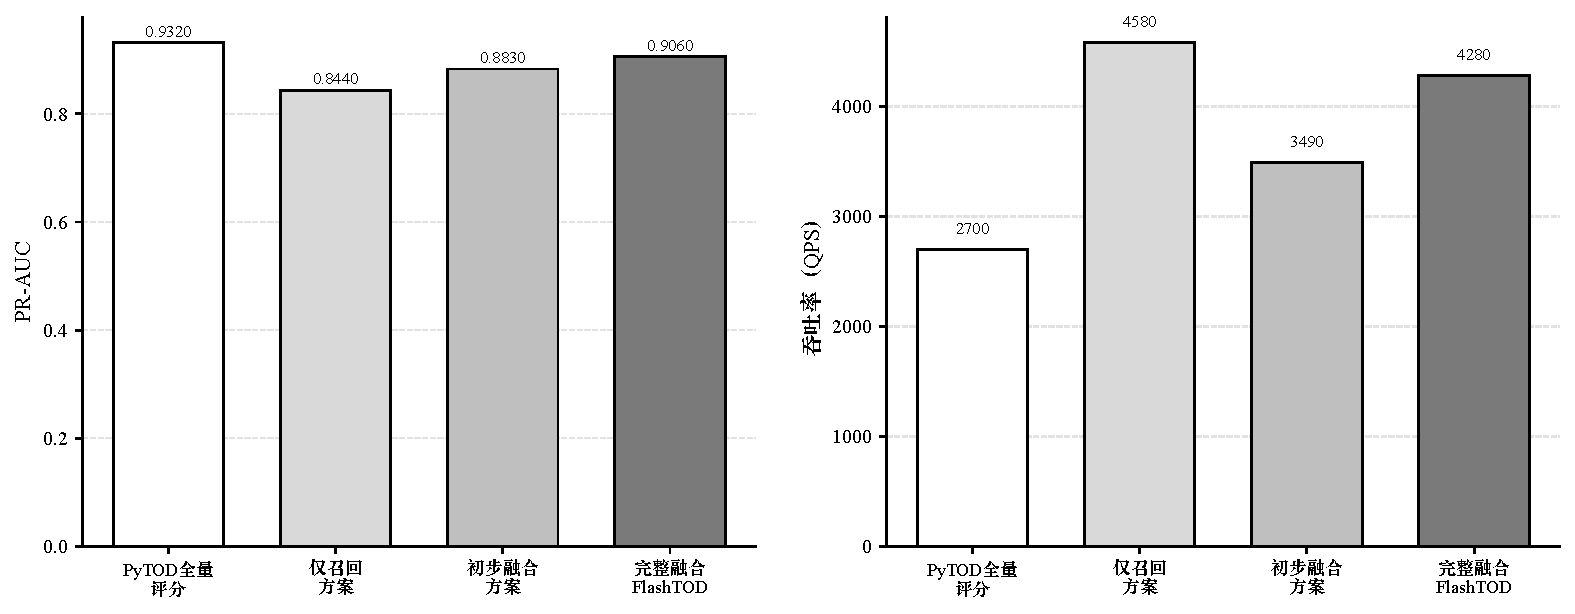
\includegraphics[width=0.95\linewidth]{figures/exp/baseline_effect_qps_comparison.pdf}
  \caption{端到端比较方案的检测效果与吞吐率（实验数据绘制）}
  \label{fig:fusion-vs-baselines}
\end{figure}

图~\ref{fig:fusion-vs-baselines}与表~\ref{tab:core-summary}使用相同的现有数据。仅召回方案吞吐最高，但 PR-AUC 为 0.844，这个内部对照只能说明召回阶段的速度上限，不能当作完整异常检测系统。FAISS-GPU + PyTOD 初步融合用于控制简单候选前端这一变量；FlashTOD 则在 FlashANNS 候选召回之外，继续组织设备侧候选和 GPU 主导数据路径。具体差异在第~\ref{sec:result-discussion}节结合路径消融结果分析。

\begin{figure}[!htbp]
  \centering
  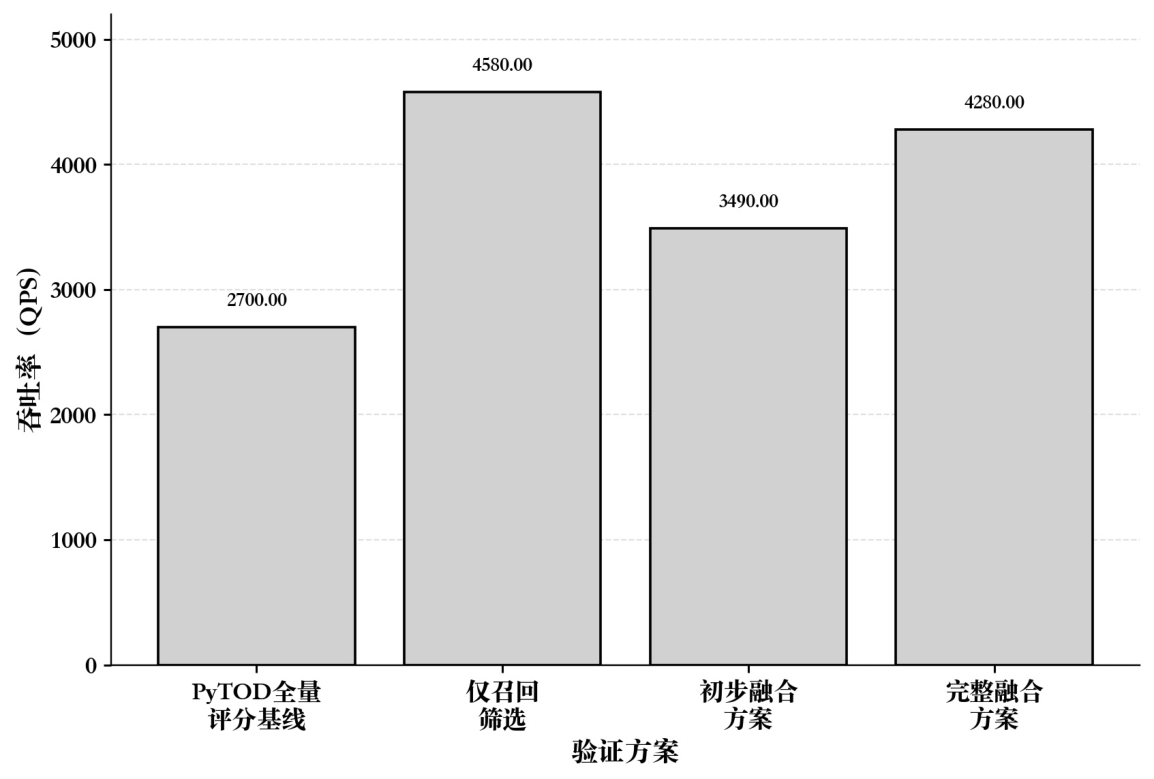
\includegraphics[width=0.8\linewidth]{plot_assets/ch06_fusion_compare/fig6_5_fusion_qps.pdf}
  \caption{端到端比较方案的吞吐率（实验数据绘制）}
  \label{fig:single-gpu-before-after}
\end{figure}

\begin{figure}[!htbp]
  \centering
  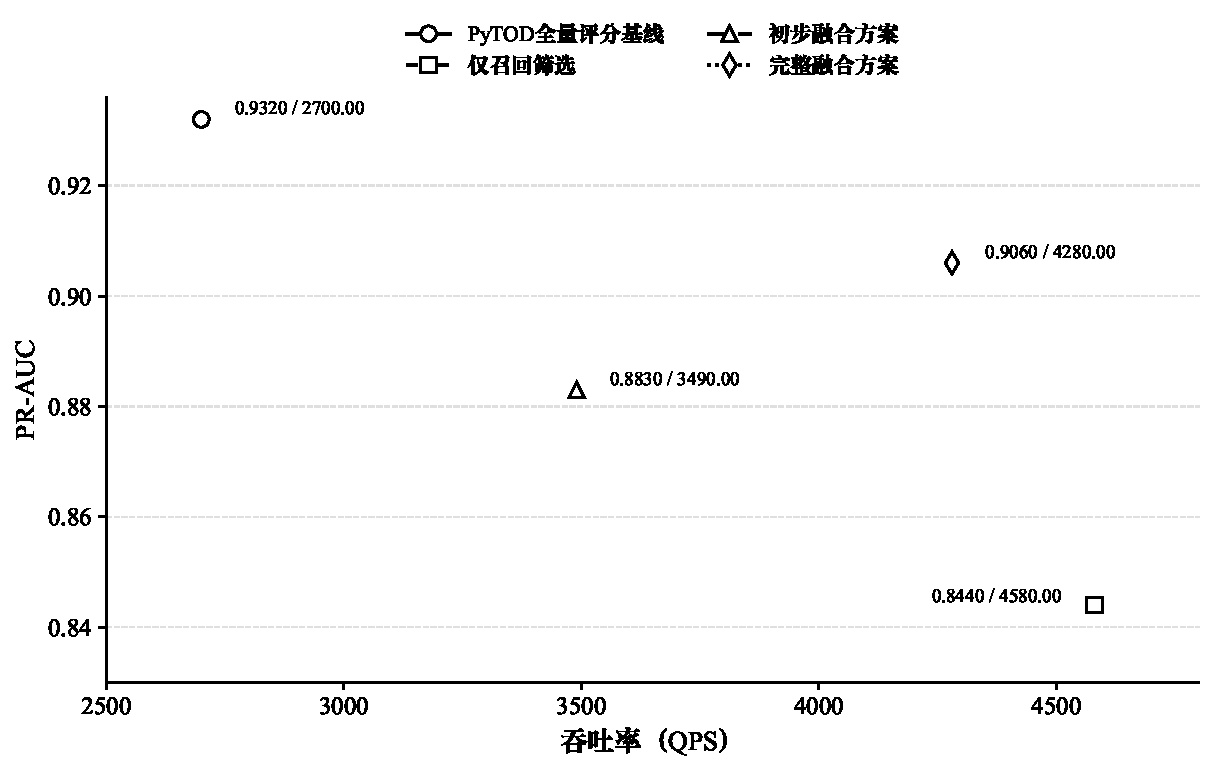
\includegraphics[width=0.82\linewidth]{plot_assets/ch06_fusion_compare/fig6_6_fusion_tradeoff.pdf}
  \caption{FlashTOD 效果与性能折中（实验数据绘制）}
  \label{fig:multi-gpu-scaling}
\end{figure}

\begin{figure}[!htbp]
  \centering
  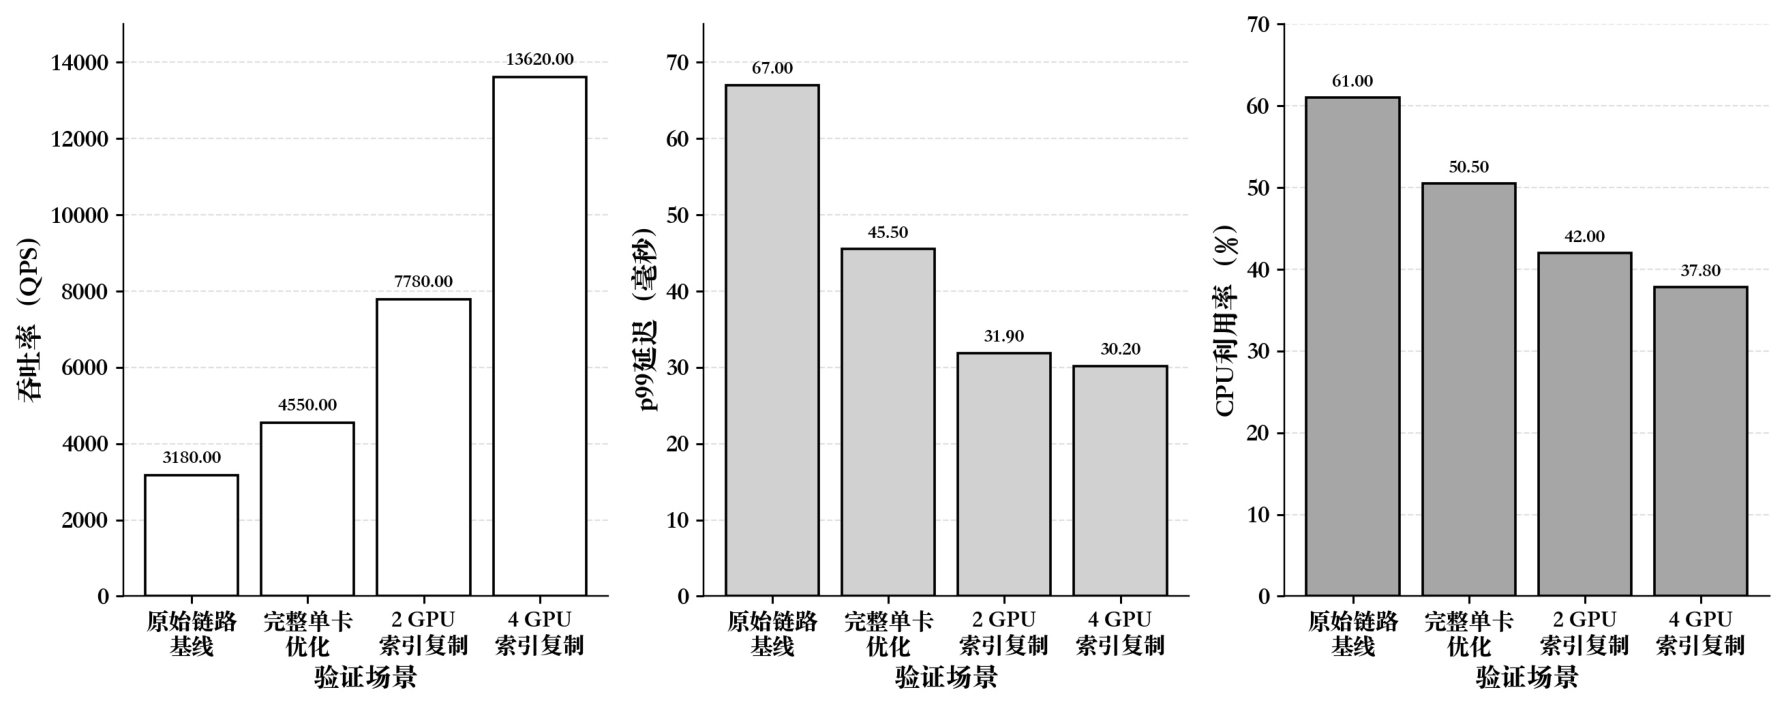
\includegraphics[width=\linewidth]{plot_assets/ch06_single_multi_summary/fig6_7_single_multi_summary.pdf}
  \caption{单卡优化与多 GPU 扩展收益对比（实验数据绘制）}
  \label{fig:scale-comparison}
\end{figure}

\begin{figure}[!htbp]
  \centering
  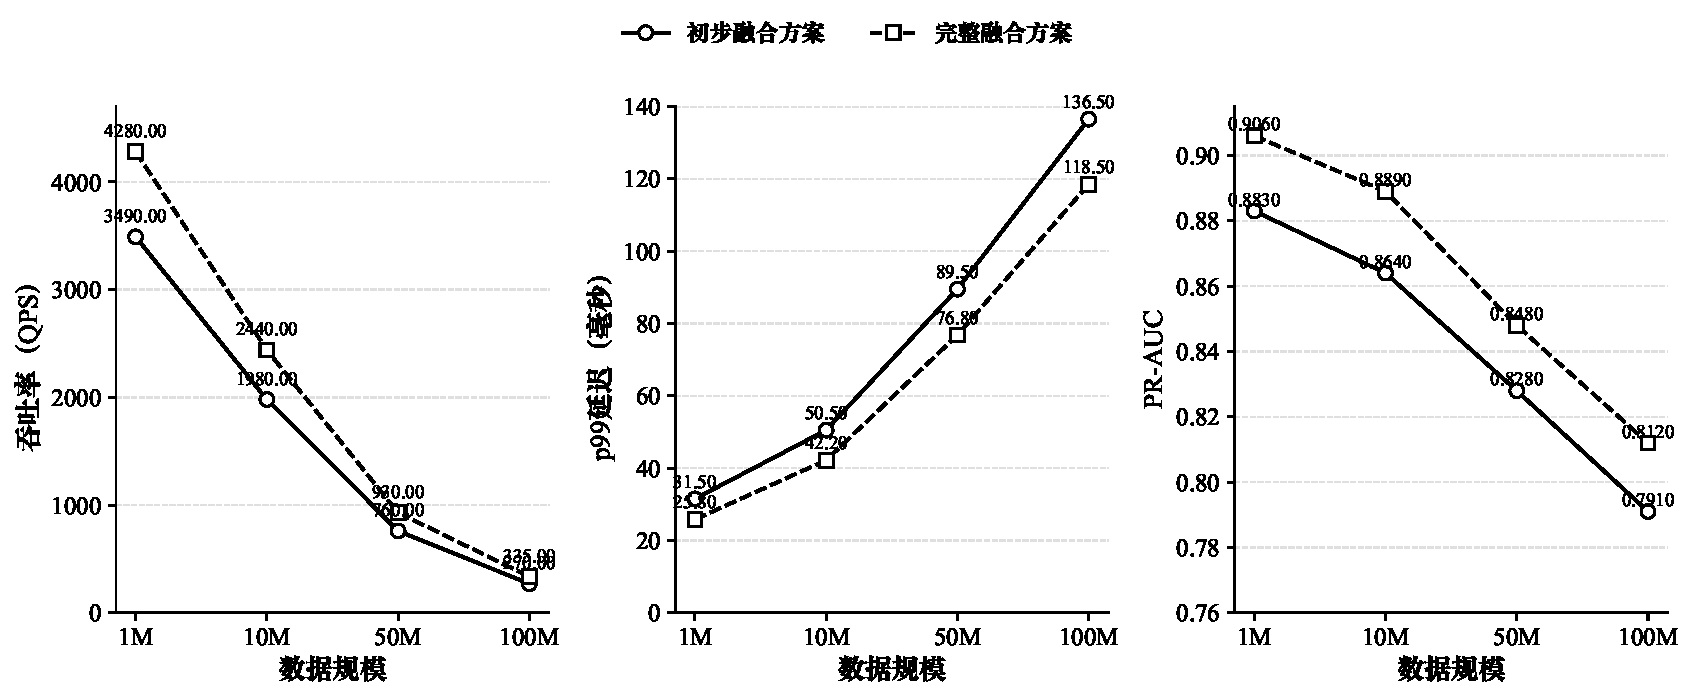
\includegraphics[width=\linewidth]{plot_assets/ch06_scale_trends/fig6_8_scale_trends.pdf}
  \caption{不同规模下系统表现趋势（实验数据绘制）}
  \label{fig:scale-trend}
\end{figure}

\section{结果讨论}
\label{sec:result-discussion}

与 PyTOD 全量评分相比，FlashTOD 改变的不是评分函数本身，而是进入高代价评分阶段的样本范围。现有结果中，PyTOD 全量评分的 PR-AUC 为 0.932、QPS 为 2700；FlashTOD 的 PR-AUC 为 0.906、QPS 为 4280。后者的吞吐率约提高 58.5\%，但 PR-AUC 下降了 0.026。因此，FlashTOD 并没有在检测效果上超过 PyTOD 全量评分。这组结果表明的是效果--效率折中：候选召回用有限的效果损失换取了更高的端到端吞吐。

FAISS-GPU + PyTOD 初步融合的 PR-AUC 为 0.883、QPS 为 3490，FlashTOD 对应为 0.906 和 4280。这一比较不能用来证明 FlashANNS 在所有条件下都优于 FAISS，因为它们面向的索引和系统问题不同。该工程组合基线只回答一个更具体的问题：把成熟 GPU ANN 接口放到 PyTOD 前面，是否已经足够。结果显示，简单串接仍未形成完整 FlashTOD 的效果与性能。

差异出现在阶段边界。候选 ID 和局部 distance 如果返回 CPU 重新打包，评分前会额外经历 D2H、CPU candidate repacking 和 H2D。后续还包含候选张量构造、GPU 中间张量驻留、阶段同步以及外存 I/O 与计算的重叠。ANN 检索本身变快，这些开销不会自动消失。FlashTOD 对设备侧候选组织和执行路径继续优化，所以该结果应解释为系统协同的收益，而不是单一 ANNS 算法的胜负。

候选召回不是全部答案。表~\ref{tab:single-gpu-benefit-source}显示，从原始分段链路到仅召回加速，QPS 由 3180 增加到 3470，p99 延迟只由 67.0~ms 降至 61.5~ms。当候选到评分的交接改为 GPU 主导路径后，QPS 进一步达到 3950，p99 降至 53.8~ms。完整优化最终将 PCIe 往返次数从每查询 6.2 降到 4.2，GPU 利用率从 48.5\% 提高到 63.5\%，p99 降至 45.5~ms，QPS 达到 4550。这是一条递进链路：候选召回解决评分范围问题，GPU 主导路径解决阶段边界问题，两者对应不同的瓶颈。

为了更清楚地解释不同优化项的收益来源，可以将端到端时间分解为
\begin{equation}
  T_{\mathrm{total}} =
  T_{\mathrm{prep}} + T_{\mathrm{retrieve}} + T_{\mathrm{pack}} +
  T_{\mathrm{score}} + T_{\mathrm{merge}} + T_{\mathrm{io}} .
  \label{eq:end-to-end-time-breakdown}
\end{equation}
式~\eqref{eq:end-to-end-time-breakdown}中，$T_{\mathrm{prep}}$表示查询准备时间，$T_{\mathrm{retrieve}}$表示候选召回时间，$T_{\mathrm{pack}}$表示候选组织与张量化时间，$T_{\mathrm{score}}$表示 PyTOD 评分时间，$T_{\mathrm{merge}}$表示多 GPU 归并时间，$T_{\mathrm{io}}$表示外存访问与主机---设备传输。候选预算主要改变 $T_{\mathrm{score}}$的输入规模，设备侧候选组织直接压缩 $T_{\mathrm{pack}}$，异步 I/O 与计算重叠减少 $T_{\mathrm{retrieve}}$ 中的等待，而多 GPU 归并会额外引入 $T_{\mathrm{merge}}$。这个分解与表~\ref{tab:single-gpu-benefit-source}中 PCIe 往返、GPU 利用率和尾延迟的同向变化一致。

多 GPU 结果回答的是另一类问题。索引可复制时，replicated 路径能直接复用单卡闭环，CPU 只需调度请求和汇总小规模结果。容量约束迫使系统分片时，GPU merge 在本文 100M 实验中的平均延迟和 p99 低于 CPU aggregation，但它仍需通信和流协调。多卡共享 PCIe/SSD 路径还会增加 I/O 排队，因此卡数增加并不等于线性扩展。

这些结果有四个明确边界。FlashTOD 的 PR-AUC 0.906 低于 PyTOD 全量评分的 0.932，效率收益并非没有代价。FAISS-GPU + PyTOD 是本文构造的工程组合基线，不是已有文献中的独立 ANN + TOD 异常检测系统。当前数据不支持将 FlashTOD 说成全面优于 HNSW、IVF/IVF-PQ 或 DiskANN。部分配置尚未覆盖完整重复运行和统计显著性检验，所以章内数值支撑的是当前实验口径下的趋势和工程取舍，不是无条件的普遍性结论。

\section{局限性分析}

超大规模实验主要依赖 IBM AML / AMLSim 等高保真合成数据。这类数据可用于施加吞吐、存储路径和多 GPU 扩展压力，却不能完全替代真实金融机构的在线负载、噪声结构和概念漂移。关于 10M、50M 和 100M 规模的结论因而限定为当前平台上的工程趋势。

PyTOD 全量评分的时间和中间结果存储开销限制了它在大规模压测中的覆盖范围。本文在 1M 桥接口径保留全量评分参考，10M 以上主要观察工程组合方案、FlashTOD 与多 GPU 内部路径。这能回答系统扩展问题，但不等同于所有规模下的全量评分横向实验。

现有对比已覆盖技术能力边界、PyTOD 全量评分参考、FAISS-GPU + PyTOD 工程组合基线以及 FlashTOD 内部路径消融。比较范围仍然有限：本文没有在相同候选预算和 PyTOD 评分后端下穷尽 HNSW、IVF/IVF-PQ 与 DiskANN 等可替换前端，也未新增 PyOD CPU 实验。所以，结论不包含对所有 ANNS 方法或异常检测系统的全面优势声称。

统计口径同样需要保留。当前数值主要来自固定硬件、查询集、候选预算和批处理参数下的已有稳定运行记录。部分配置尚未提供完整重复轮次、标准差、误差棒和显著性检验，因此章内差异用于趋势性比较和工程可行性分析，不解释为统计显著结论。

多 GPU 主方案也有适用前提。replicated 依赖索引可复制；索引超出单卡容量后必须转向 sharded 路径，并承担通信与归并代价。外存和拓扑感知 I/O 收益还取决于 GPU--SSD--PCIe--NUMA 拓扑、驱动与 GDS 支持。本文只验证单机多 GPU，多机通信、分布式索引与集群调度尚未进入实验范围。

\section{本章小结}

本章的综合实验把全文前几章分散建立的判断收束到同一验证框架中。在本文设定的数据规模、硬件平台和候选预算条件下，FlashTOD 在保持合理检测效果的同时，体现出面向大规模金融异常检测的系统组织价值；单卡优化的主要收益来自候选召回到异常评分之间的数据路径压缩；多 GPU 条件下，索引复制可作为吞吐优先场景的主方案，而设备侧归并与拓扑感知 I/O 控制则主要用于容量受限或路径受限场景下维持扩展效果。
